\chapter{Machine Learning in Multi-Agent Systems}
\label{chap:farm}

One of the outstanding challenges in ABMs of coupled natural and human systems 
concerns the lack of ABMs to simulate agents with the ability to learn from 
their past failures or successes and environmental and social uncertainties.
\cite{sert2020segregation}

\section{Methodology}
\label{sec:farm_methods}

\subsection{Problem Definition}
\label{subsec:farm_methods_problem}

\subsection{Modeling Approach}
\label{subsec:farm_methods_approach}

The deep reinforcement machine learning methods being used in this model are
based on the deep q-learning methods developed by Hasselt, Guez, and
Silver\cite{ddqn16}, incorporating some of the alterations to action replay
and learning convergence as described in the rainbow algorithm developed by
Hesel et al.\cite{rainbow18}

\subsection{Agent Decision-Making}
\label{subsec:farm_methods_decisions}

Agents in this model make decisions according to an internal decision-policy
function $\pi(s)=a$ mapping the state of each agent to the potential actions 
that each agent can take.
In this approach, the decision-policy function is being approximated by
an artificial neural network (ANN), $\mu:S\rightarrow A$.
The input to this ANN is the state of the agent, vectorized as a 1-dimensional
array of length $W_S$.
The output of the ANN is a vector of length $W_A$ encoding the action that
the ANN has decided the agent should take.

\subsection{Agent Learning}
\label{subsec:farm_methods_learning}

\subsection{Agent Memory}
\label{subsec:farm_methods_memory}

Agents in the model store a history of their past experience as
a series of state transition records $(s_t,a_t,r_t,s_{t+1})$.
These records are stored in a memory buffer $B$ of fixed length $N$.
When the memory buffer is full, new records overwrite the oldest records in
the buffer.
The memory buffer is used to train the agent's decision-policy 

\section{Experimental Design}
\label{sec:farm_exp}

\subsection{Simulation Environment}
\label{subsec:farm_exp_env}

In order to test this modeling methodology,
an experimental agent-based model was developed to explore the behavior
of a multi-agent system of agricultural decision-makers
and how that behavior may change in response to various external stimuli.
The real-world basis for this model is a study area in the
Missisquoi Bay Area of the Lake Champlain Basin of Vermont,
and the model is designed to represent the agricultural decision-making
processes of farmers in this area.
In particular, decisions pertaining to land use practices and
the adoption or rejection of agricultural best management practices (BMPs)
were studied.

The model was implemented using the FLAMEGPU framework (FLAMEGPU),
which is an agent-based modeling framework that allows for the
development of models that can be run on a GPU-device,
and with CUDNN (CUDNN),
a deep learning library for CUDA.
These technologies were selected \textbf{EXPAND RATIONALE}

\subsubsection{Agents}
\label{subsubsec:farm_exp_agent}

There are two types of agents present in this model --- 480 farmer agents, 
corresponding to the 480 agriculturally-zoned land parcels in the Missisquoi 
Bay Area, 
and a single regulatory agent.
All agents in the model contain some internal information about their current 
state and history, a set of state-transition memories used to learn from 
experience, and a pair of neural networks used to drive agent decision-making. 
As the agents make decisions over time, they gradually learn the correlation 
between the actions they take from each state using deep reinforcement machine 
learning.

The 480 farmer agents are used to model the behavior of agricultural land 
managers within the study area. 
These agents make annual decisions, once per time-step, 
about their farming practices, 
including whether they should adjust their productivity in one of four 
agricultural sectors (beef, dairy, corn, and hay) 
and whether they should implement an agricultural best management practice 
(BMP) to reduce phosphorus on their land.

Conditions that factor in as components of a farmer agent's state include the 
total land area the agent has devoted to cropland or pasture; 
the productivity of the agent in each of the four modeled agricultural 
industries along with their associated phosphorus byproduct productivity; 
an n-year history of the farm's profitability, storm losses, and BMP usage; 
and similar historical information from the agent's k-nearest neighboring
farmer agents.

The one municipal regulatory agent is used to model a municipal government or 
regulatory agency's behavior managing agricultural practices on the landscape 
and the local environment and the policies that guide them. 
This agent acts more slowly than the agricultural agents, 
once every five time-steps, and decides if/how it should modify its incentive 
structure --- changing its taxation rate, the subsidization given to an agent 
adopting a BMP, and the phosphorus runoff threshold at which a penalty is 
applied.

The municipal regulatory agent's state conditions include a history of 
extreme weather events in the region; and the aggregate profitability, 
phosphorus runoff, and storm loss across the last five time-steps for all 
agents.

\subsection{Hyperparameter Selection}
\label{subsec:farm_exp_hyper}

A summary of model hyperparameters is listed in Table~\ref{tab:farm_exp_hyper}.

Preliminary model runs were conducted to determine the optimal values for
the hyperparameters for machine learning within the model.
The learning hyperparameters that were varied in these preliminary runs were
the number of training episodes,
the number of steps between target network updates,
the number of inner layers in the neural networks,
the number of neurons in each of those inner layer,
the learning rate,
and the batch size.
The learning hyperparameters that were held constant were
the exploration rate at $\varepsilon = 0.1$,
the discount factor at $\gamma = 0.99$,
the learning transfer rate at $\tau = 0.001$,
the number of steps within a training episode at $N = 40$,
the replay memory size at $M = 10000$.

A summary of the final model hyperparameters are listed in
Table~\ref{tab:farm_exp_hyper}.
Network-specific parameters are listed in Table~\ref{tab:farm_exp_nets}.

\begin{table}
\centering
\caption{Hyperparameters and associated values with source or rationale
    for the agricultural land use model}
\label{tab:farm_exp_hyper}
\begin{tabular}{lll}
\hline
Parameter & Value & Source/Rationale \\
\hline
    Learning Rate ($\alpha$) & 0.00025 & \\
    Exploration Rate ($\varepsilon$) & 0.1 & \\
    Discount Factor ($\gamma$) & 0.99 & \\
    Transfer Rate ($\tau$) & 0.001 & cite \emph{Transfer learning} \\
    Replay Memory Size ($M$) & 10000 & \\
    Batch Size ($B$) & 32 & \cite{ddqn16} \\
%    Target Network Update Frequency ($f$) & & \\
    Number of Episodes ($N$) & 1000 & Testing \textbf{Expand} \\
    Number of Steps per Episode ($T$) & 40 
    & Econ model limitations \textbf{Expand} \\
\hline
\end{tabular}
\end{table}

\begin{table}
\centering
\caption{Network parameters for the ANNs used by the agents in the agricultural
land use model, where the $\mu_a$ and $Q_a$ columns correspond to the values
for the agricultural agents' networks and $\mu_r$ and $Q_r$ 
correspond to the values for the regulatory agent networks
\textbf{Include bias line?}}
\label{tab:farm_exp_nets}
\begin{tabular}{lllll}
    \hline
    Parameter & $\mu_a$ & $Q_a$ & $\mu_r$ & $Q_r$ \\
    \hline
    Input Nodes & 15 & 32 & 12 & 22 \\
    Inner Layers & 5 & 5 & 5 & 5 \\
    Inner Nodes & 10 & 16 & 10 & 16 \\
    Activation Function & ReLU & ReLU & ReLU & ReLU \\
    Connectivity & Full & Full & Full & Full \\
    Output Nodes & 17 & 1 & 5 & 1 \\
    Output Activation & $n$-hot & Linear & $n$-hot & Linear \\
    Output Groups ($n$) & 5 & --- & 3 & --- \\
    \hline
\end{tabular}
\end{table}

\subsection{Experimental Setup}
\label{subsec:farm_exp_setup}

The model was run for a variety of scenarios.
All scenarios tested the variables $BMP_e$, $\Delta EE$,
and $g$.
Then, there were two classes of test:
tests with agents with uniform memory accuracy (Table~\ref{tab:farm_exp_par})
and tests with agents with heterogeneous memory accuracy
(Table~\ref{tab:farm_exp_mix}).

BMP Efficacy ($BMP_e$) was varied from 0.0 to 1.0 in increments of 0.1.
This parameter represents the effectiveness of BMPs in reducing nutrient
loading from agricultural fields.
A value of 0.0 indicates that BMPs have no effect on nutrient loading,
while a value of 1.0 indicates that BMPs completely eliminate nutrient loading.
This parameter was varied in order to determine the effect of BMP efficacy
on the behavior of the system.

Change in weather event frequency ($\Delta EE$) was varied from -0.2
to 0.2 in increments of 0.05.
This parameter represents the change in the frequency of extreme weather
events, such as heavy rainfall, that may be induced by climate change
compared to a historical baseline.

\textbf{Change verbiage from threshold to scale?}
The regulation change threshold ($g$) represents the maximum rate at which
the regulatory agent will adjust the regulatory environment.
Three values were tested: an aggressive threshold ($g=0.2$),
a moderate threshold ($g=0.05$), and
a restrictive case ($g=0$) for testing the model's ability to
operate in a static regulatory environment.

\textbf{Change wording: $F'$ for accuracy and $F$ for forgetfulness is bad.}
The impact of agent memory accuracy was tested for two types of agent
populations.
In uniform agent populations, all agents had the same memory recall
accuracy ($F'$), where $F'$ is the probability that a memory will be
recalled correctly.
In heterogeneous agent populations, agents had different memory recall
accuracies, 
where a proportion of agents ($P$) had accuracy $F=1$
and all other agents ($1-P$) had accuracy $F=0$.

\begin{table}
\centering
\caption{Table listing experimental parameters for uniform population runs}
\label{tab:farm_exp_par}
\begin{tabular}{ll}
\hline
Variable & Values \\
\hline
BMP Efficacy ($BMP_e$) & 0, 0.1, 0.2, 0.3, 0.4, 0.5, 0.6, 0.7, 0.8, 0.9, 1.0 \\
Change in Event Frequency ($\Delta EE$)
    & -0.2, -0.15, -0.1, -0.05, 0.0, 0.05, 0.1, 0.15, 0.2 \\
Regulation Change Threshold ($g$)
    & 0, 0.05, 0.2 \\
Recall Accuracy ($F'$) & 0, 0.25, 0.5, 0.75, 1 \\
\hline
\end{tabular}
\end{table}

\begin{table}
\centering
\caption{Table listing experimental parameters for mixed population runs}
\label{tab:farm_exp_mix}
\begin{tabular}{ll}
\hline
Variable & Values \\
\hline
BMP Efficacy ($BMP_e$) & 0, 0.1, 0.2, 0.3, 0.4, 0.5, 0.6, 0.7, 0.8, 0.9, 1.0 \\
Weather Event Frequency ($\Delta EE$)
    & -0.2, -0.15, -0.1, -0.05, 0.0, 0.05, 0.1, 0.15, 0.2 \\
Regulation Change Threshold ($g$)
    & 0, 0.05, 0.2 \\
Population Mixing ($P$) & 0.25, 0.5, 0.75 \\
\hline
\end{tabular}
\end{table}

\section{Results}
\label{sec:farm_results}

\subsection{Model Performance}
\label{subsec:farm_results_robust}

For each model parameterization,
agents were trained for 1000 training episodes.
If more than 10\%  of the agents ($n=48$) in the model failed to converge
to a stable policy within 1000 training episodes, the model was discarded 
and retrained; however, this occurred in less than 2\% of model runs.
A plot showing the distribution of number of agents which converged
across model parameterizations is shown in Figure~\ref{fig:farm_sfc}.

\begin{figure}
\centering
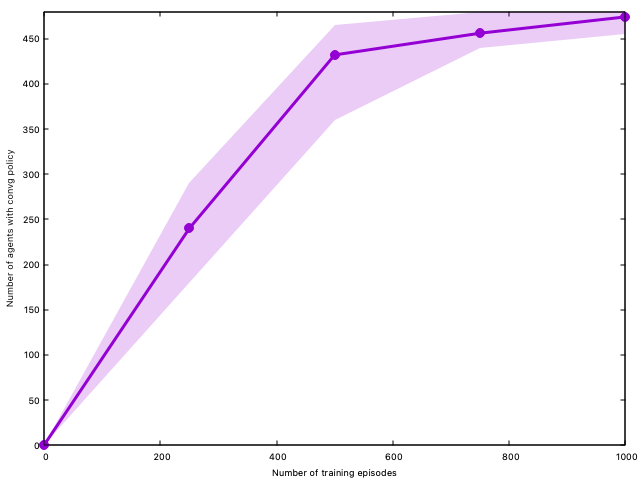
\includegraphics[width=.4\textwidth]{figure/sfc}
\caption{Plot of the number of agents that converged to a stable policy
    for each parameterization of the model}
\label{fig:farm_sfc}
\end{figure}

Models which were successfully trained and passed through this screening
were then run for 40 testing runs.

\subsection{Agent Behavior}
\label{subsec:farm_results_agents}

\subsubsection{Uniform Population Runs}

For model parameterizations with uniform agent populations,
the proportion of agents which adopted a BMP in each testing model run
was recorded and used to generate a distribution of BMP adoption rates
for each parameterization.
Summaries of the results of these runs are shown
in Figure~\ref{fig:farm_res_g00} for the case where the regulation change
threshold ($g$) was set to 0.0,
Figure~\ref{fig:farm_res_g05} for when $g$ was set to 0.05, and 
Figure~\ref{fig:farm_res_g20} for when $g$ was set to 0.2.

Some parameterizations have been omitted for readability.
The full listing of results can be found in
Appendix~\ref{app:results}.

\begin{figure}
    \subcaptionbox{$F=0$}{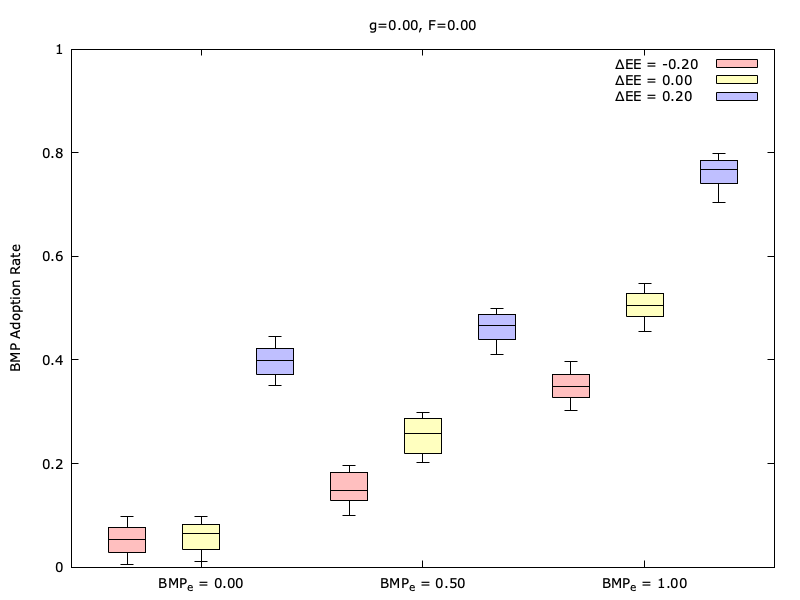
\includegraphics[width=.3\textwidth]{figure/g0F0}}
    \hfill
    \subcaptionbox{$F=0.5$}{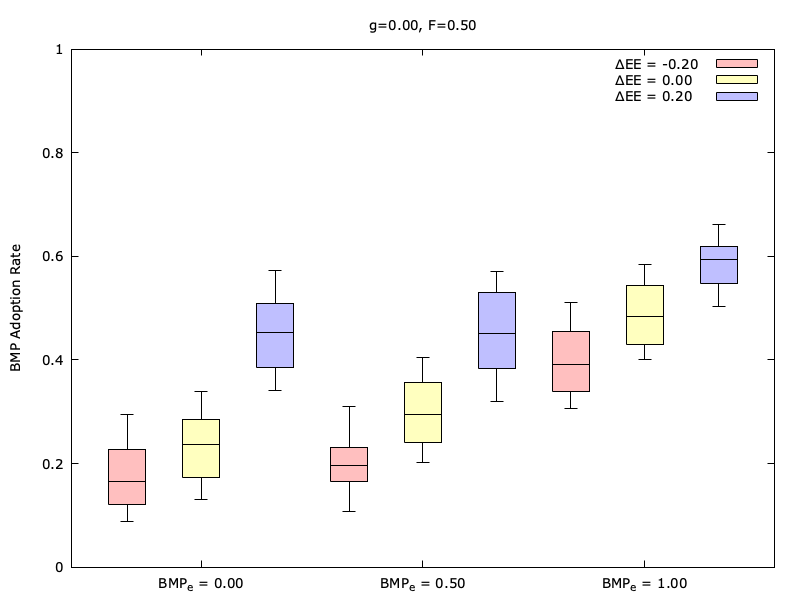
\includegraphics[width=.3\textwidth]{figure/g0F05}}
    \hfill
    \subcaptionbox{$F=1.0$}{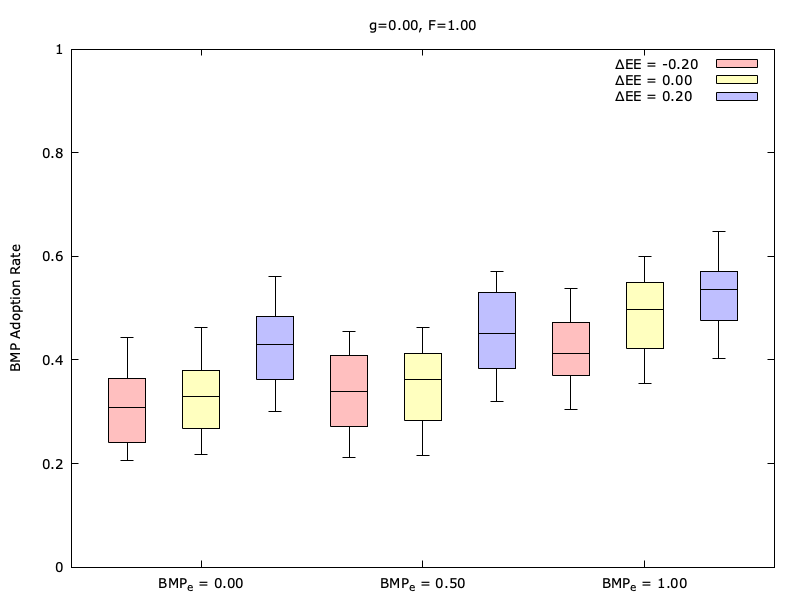
\includegraphics[width=.3\textwidth]{figure/g0F10}}
    \caption{Distribution of mean BMP adoption rate for uniform population
        runs of the agricultural land use model, where $g=0.0$,
        for (a) $F=0$, (b) $F=0.5$, and (c) $F=1.0$}
    \label{fig:farm_res_g00}
\end{figure}

\begin{figure}
    \subcaptionbox{$F=0$}{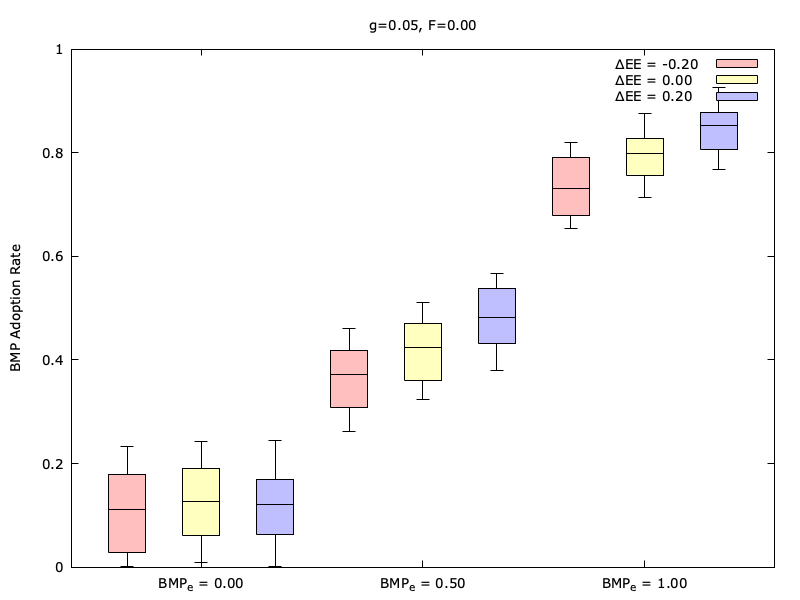
\includegraphics[width=.3\textwidth]{figure/g05F0}}
    \hfill
    \subcaptionbox{$F=0.5$}{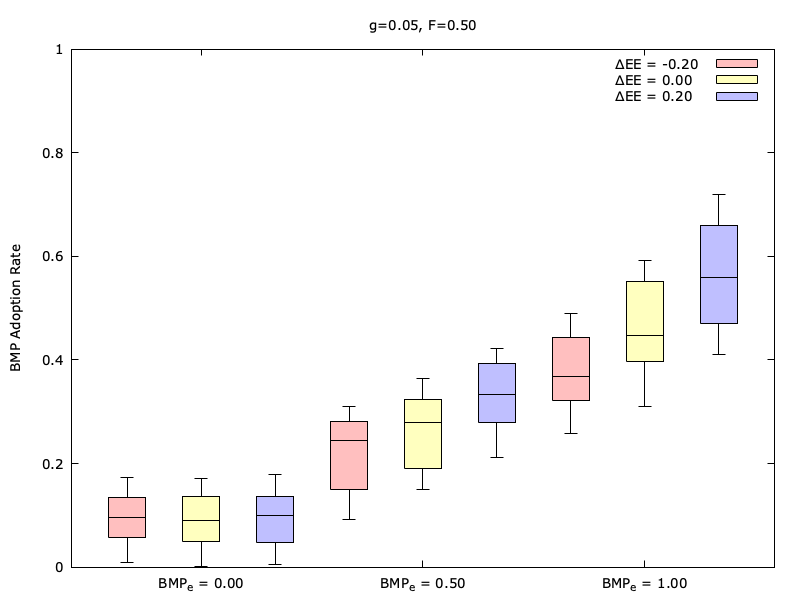
\includegraphics[width=.3\textwidth]{figure/g05F5}}
    \hfill
    \subcaptionbox{$F=1.0$}{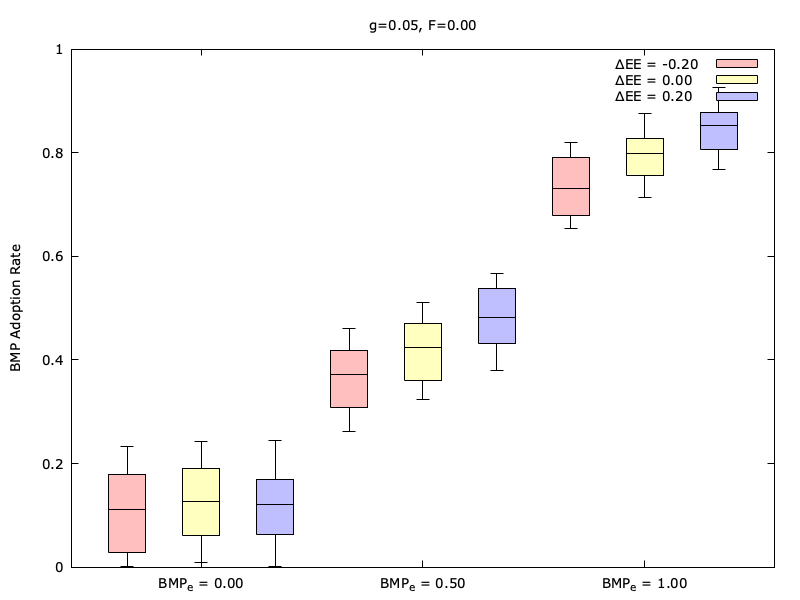
\includegraphics[width=.3\textwidth]{figure/g05F0}}
    \caption{Distribution of mean BMP adoption rate for uniform population
        runs of the agricultural land use model, where $g=0.05$,
        for (a) $F=0$, (b) $F=0.5$, and (c) $F=1.0$}
    \label{fig:farm_res_g05}
\end{figure}

\begin{figure}
    \subcaptionbox{$F=0$}{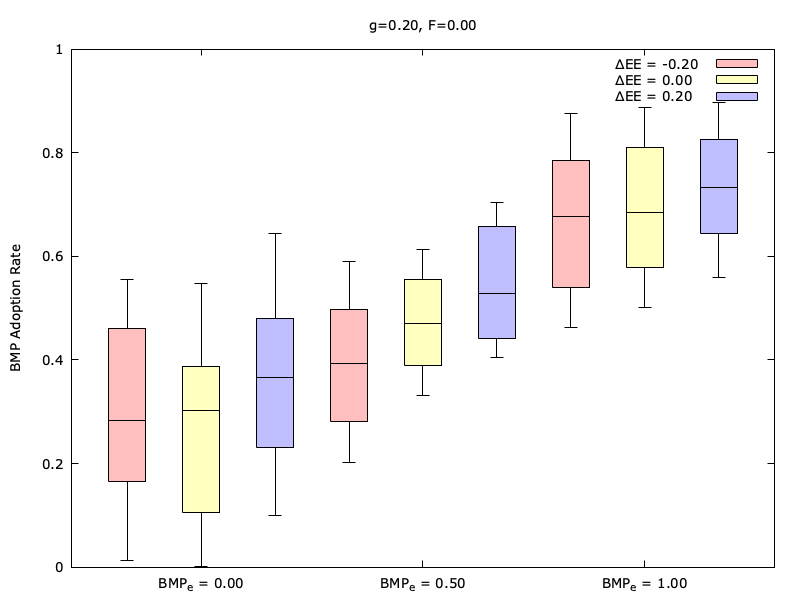
\includegraphics[width=.3\textwidth]{figure/g20F0}}
    \hfill
    \subcaptionbox{$F=0.5$}{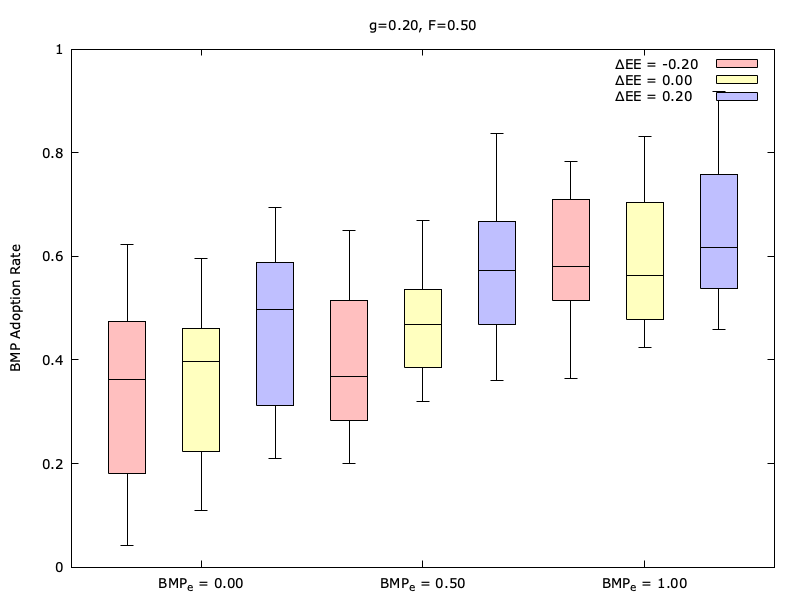
\includegraphics[width=.3\textwidth]{figure/g20F05}}
    \hfill
    \subcaptionbox{$F=1.0$}{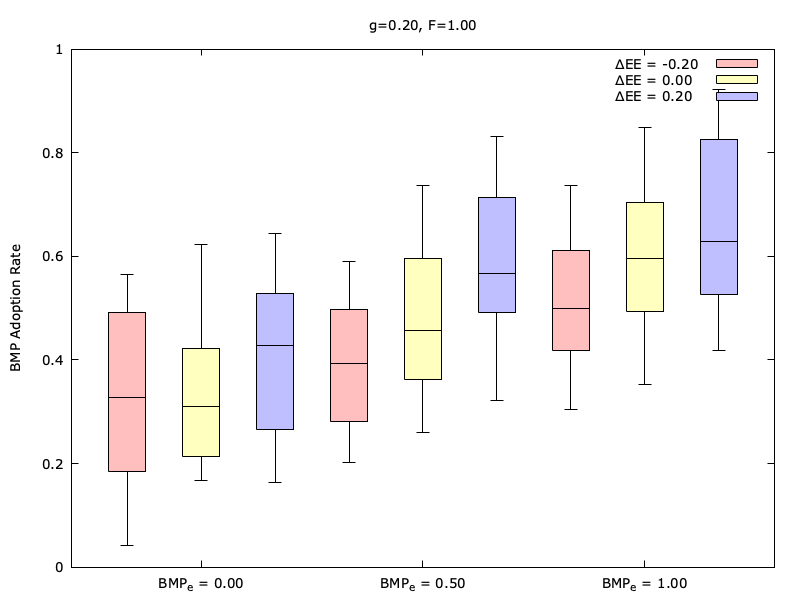
\includegraphics[width=.3\textwidth]{figure/g20F10}}
    \caption{Distribution of mean BMP adoption rate for uniform population
        runs of the agricultural land use model, where $g=0.2$,
        for (a) $F=0$, (b) $F=0.5$, and (c) $F=1.0$}
    \label{fig:farm_res_g20}
\end{figure}

\subsubsection{Mixed Population Runs}

For model parameterizations with mixed agent populations,
agents were divided into three groups:
group 1, where $F=0$ for the agent and all neighbors,
group 2, where $F=1$ for the agent and all neighbors, and
group 3, for agents with neighbors where $F=0$ and $F=1$. 
The proportion of agents in each group which adopted a BMP in each testing
model run was recorded and used to generate a distribution of BMP adoption
rates for each parameterization.
Results of one set of parameterizations of these runs are shown
in Figure~\ref{fig:farm_res_mix0} where $g=0$, $\Delta EE=0$.
The results indicate generally that this method of introducing
heterogeneity into the population can introduce variance in
agent behavior, but that it is unclear if it leads to any
of the desired emergent behavioral patterns.
Further testing, specifically targeting these types of populations
would be needed to draw stronger conclusions.

A full table listing the results for all parameterizations can
be found in Table~\ref{tab:full_res_mixed}.

\begin{figure}
    \subcaptionbox{$P=0.25$}{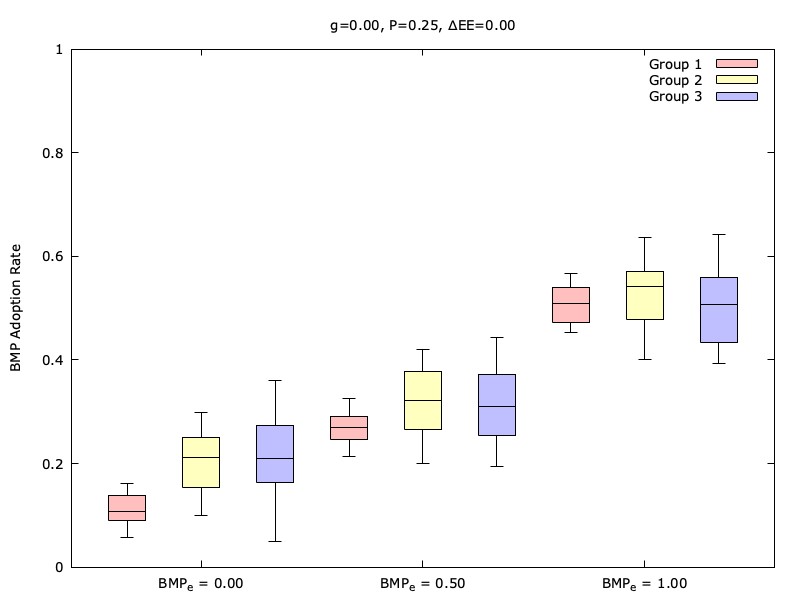
\includegraphics[width=.3\textwidth]{figure/g0P25}}
    \hfill
    \subcaptionbox{$P=0.5$}{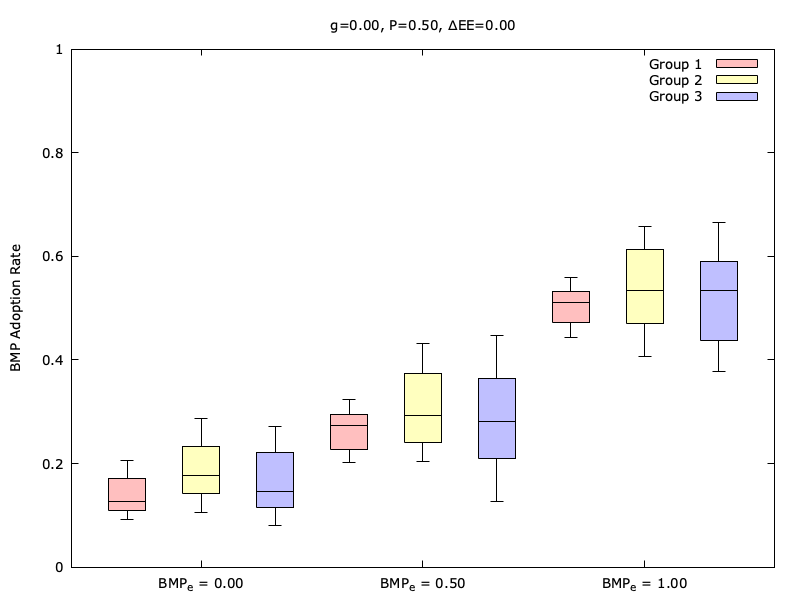
\includegraphics[width=.3\textwidth]{figure/g0P50}}
    \hfill
    \subcaptionbox{$P=0.75$}{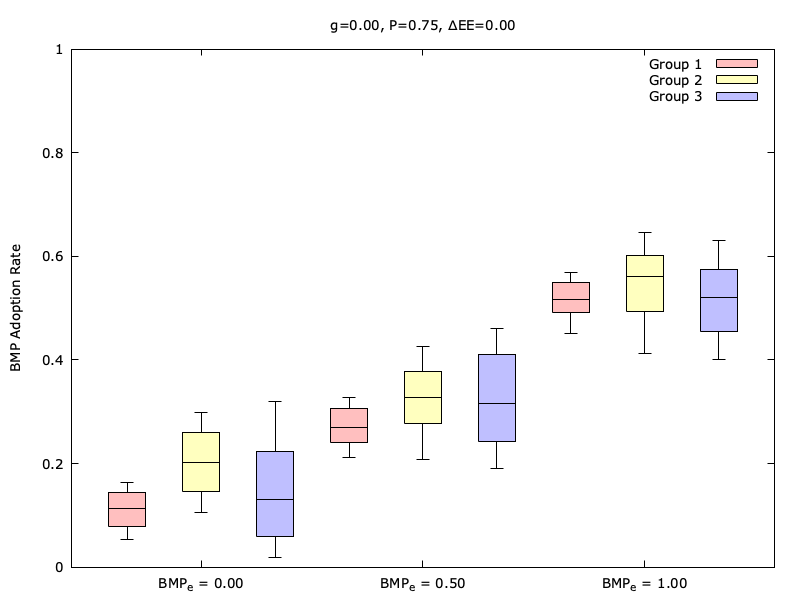
\includegraphics[width=.3\textwidth]{figure/g0P75}}
    \caption{Distribution of mean BMP adoption rate for mixed population
        runs of the agricultural land use model, where $g=0.0$,
        $\Delta EE=0$,
        for (a) $P=0.25$, (b) $P=0.5$, and (c) $P=0.75$}
    \label{fig:farm_res_mix0}
\end{figure}

\section{Discussion}
\label{sec:farm_disc}

\subsection{Sensitivity and Limitations}

The purpose of the regulatory agent was to help incentivize agent learning,
but in results with $g=0.2$, the increased variability in model performance
was high and the impact dominated all other parameters.
\textbf{Detail, Scaling in results, mean and variance, why these results
even matter}

